\chapter{External Simulink Models}
\label{MMSimulink}
The TLM plugin has been implemented for Simulink. 
This section describes how to use and install the plugin to be able to integrate Simulink models into composite models and co-simulations.

\section{TLM Simulink Library}
\label{sec:TLMLib}
A Simulink library exists that contains different Simulink blocks, see also Figure~\ref{fig:TLMLib}. 
The main block is the {\tt TLMForce} block that is a Simulink S-Function implementation of the TLM plugin. 
The {\tt TLMDriver} and {\tt TLMInterface} are subsystems that are used to connect SimMechanics components to the {\tt TLMForce}. 
Additionally, some useful Simulink blocks are collected in the {\tt TOOLS} sub-system, for instance, blocks for matrix transformations.

\begin{figure}[ht]\begin{center}
   {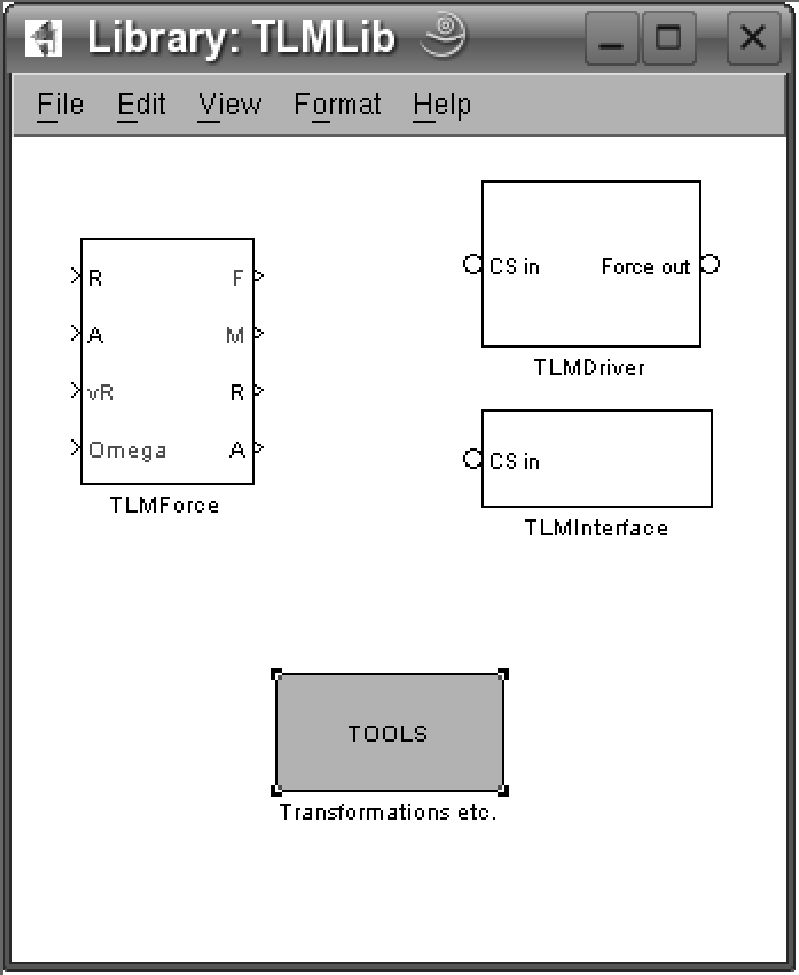
\includegraphics[width=4cm]{figs/TLMLib.png}}
    \caption{The Simulink TLM library for coupled simulations.}
    \label{fig:TLMLib}
\end{center}\end{figure}

The ({\tt TLMForce}) block takes four input variables: position ({\tt R}), orientation matrix ({\tt A}), velocity ({\tt vR}), and rotational velocity ({\tt Omega}). 
TLM calculates output force ({\tt F}) and moment ({\tt M}) from velocity and rotational velocity. 
From a TLM point of view, the most important variables are {\tt vR} and {\tt Omega}. 

Position and orientation are mainly used for graphics in the composite model editor (CME) and for possible coordinate transformations. 
All input data must be expressed relative the inertial coordinate system of the simulation model. 
All output data is expressed relative the inertial coordinate system of the simulation model.

Position, velocities, force, and moment, are vectors of dimension three: [X Y Z]. 
Whereas the orientation matrix is a vectors of dimension nine defining the 3x3 matrix A(row, column): [A(1,1) A(1,2) A(1,3) A(2,1) A(2,2) A(2,3) A(3,1) A(3,2) A(3,3)]


\section{Test Case: Pendulum}
A pendulum with three TLM connected shafts has been implemented as a test model, see Figure~\ref{fig:Shafts}. 
Each shaft is modeled as a separate Simulink model using SimMechanics.

\begin{figure}[ht]\begin{center}
   {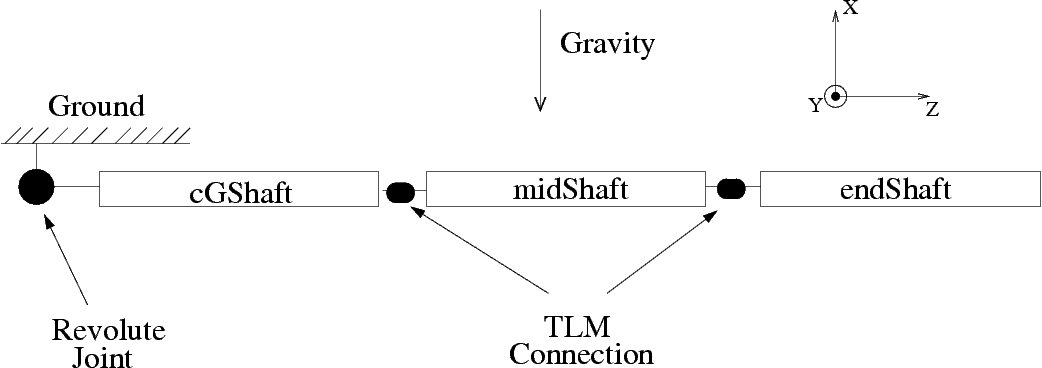
\includegraphics[width=8cm]{figs/Shafts.png}}
    \caption{Three shaft pendulum with TLM connections between the
	shafts and a revolute joint connected to the ground.}
    \label{fig:Shafts}
\end{center}\end{figure}

The Simulink model of the three shaft pendulum has been implemented with SimMechanics and the {\tt TLMInterface} from the TLMLib, see also Section~\ref{sec:TLMLib}. 
cGShaft is connected to the ground using a {\tt Revolute} joint from the SimMechanics library, see Figure~\ref{fig:cGShaft}. 
The other shafts (midShaft and endShaft) are based on a Simulink model with a free body using a {\tt Six-DoF} joint, see Figure~\ref{fig:Shaft}. 
All three shafts are connected in their TLM interfaces.

\begin{figure}[ht]
\centering
\subfigure[SimMechanics shaft connected to ground with revolute joint.]{
   	{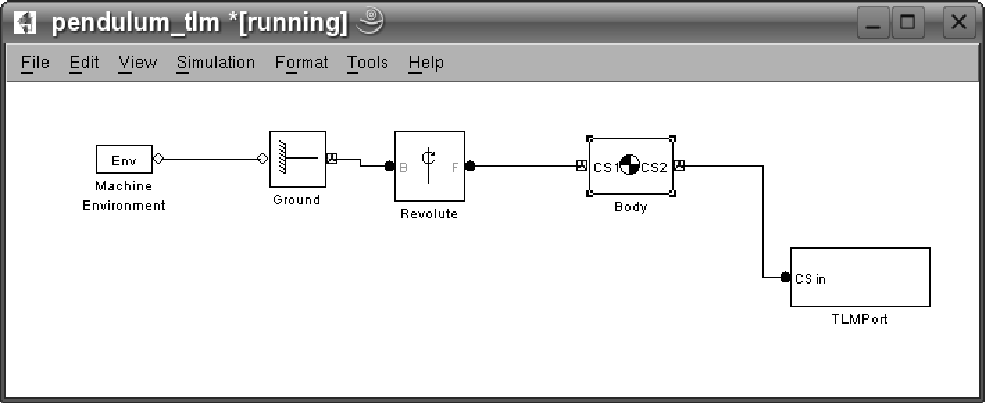
\includegraphics[width=8cm]{figs/SimulinkcGShaft.png}}
	\label{fig:cGShaft}
	}
\subfigure[Free SimMechanics shaft model.]{
   	{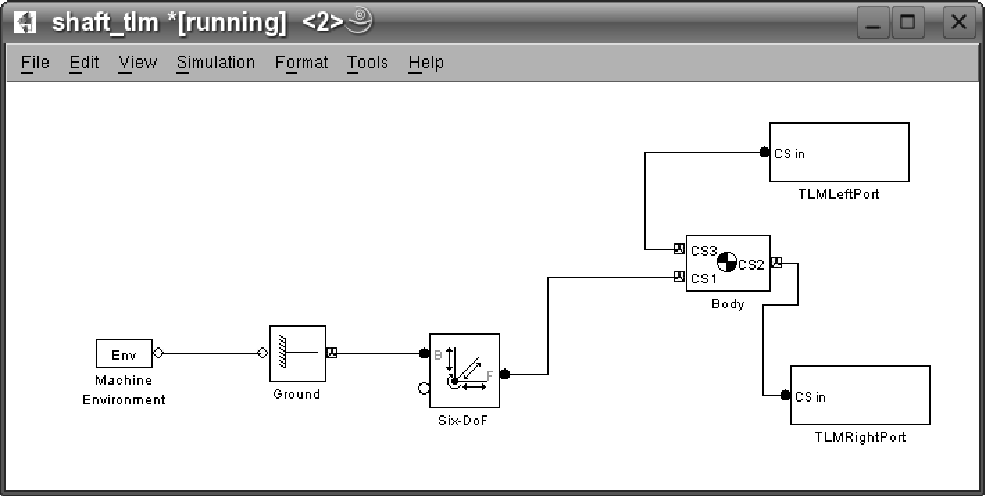
\includegraphics[width=8cm]{figs/SimulinkShaft.png}}
	\label{fig:Shaft}
     	}	
\caption{Simulink SimMechanics models for the three shaft pendulum.}
\label{fig:surfData}
\end{figure}

Each of the shafts has a mass of {\tt 3Kg}, a length of {\tt 160mm}, and a diameter of {\tt 40mm}. 
Assuming that the characteristic length $L_0$ is equal to the diameter of the shaft we can calculate the TLM parameters for the model according to Section~\ref{secTLMtheory}, as follows:

\begin{equation}
\begin{array}{l}
T_{TLM} =  0.04/5180 \approx 8*10^{-6} \\
\\
Z_F =  210*10^{9} * 0.04 * 8*10^{-6} \approx 68000 \\
\\
Z_{FR} =  \frac{1}{4}*68000*0.04^2 \approx 30
\end{array}
\end{equation}

The composite model describes how the shafts are connected and what TLM parameters should be used in the different TLM connections. 
It is created using the composite model Editor.
%, see Figure~\ref{fig:MMShafts}.

The pendulum model is simple and has all important characteristics to test the TLM plugin:
\begin{itemize}
\item Multiple simulation models with single and multiple TLM interfaces and connections.
\item Open (not connected) TLM interface in the endShaft.
\item Translational displacement of the midShaft and endShaft.
\item Rotational and translational motion.
\end{itemize}

Results from the co-simulation can be verified by plotting the movement of the TLM interfaces.

\begin{figure}[ht]
\centering
\subfigure[Moment in TLM connected coordinate systems cGShaft-midShaft.]{
   	{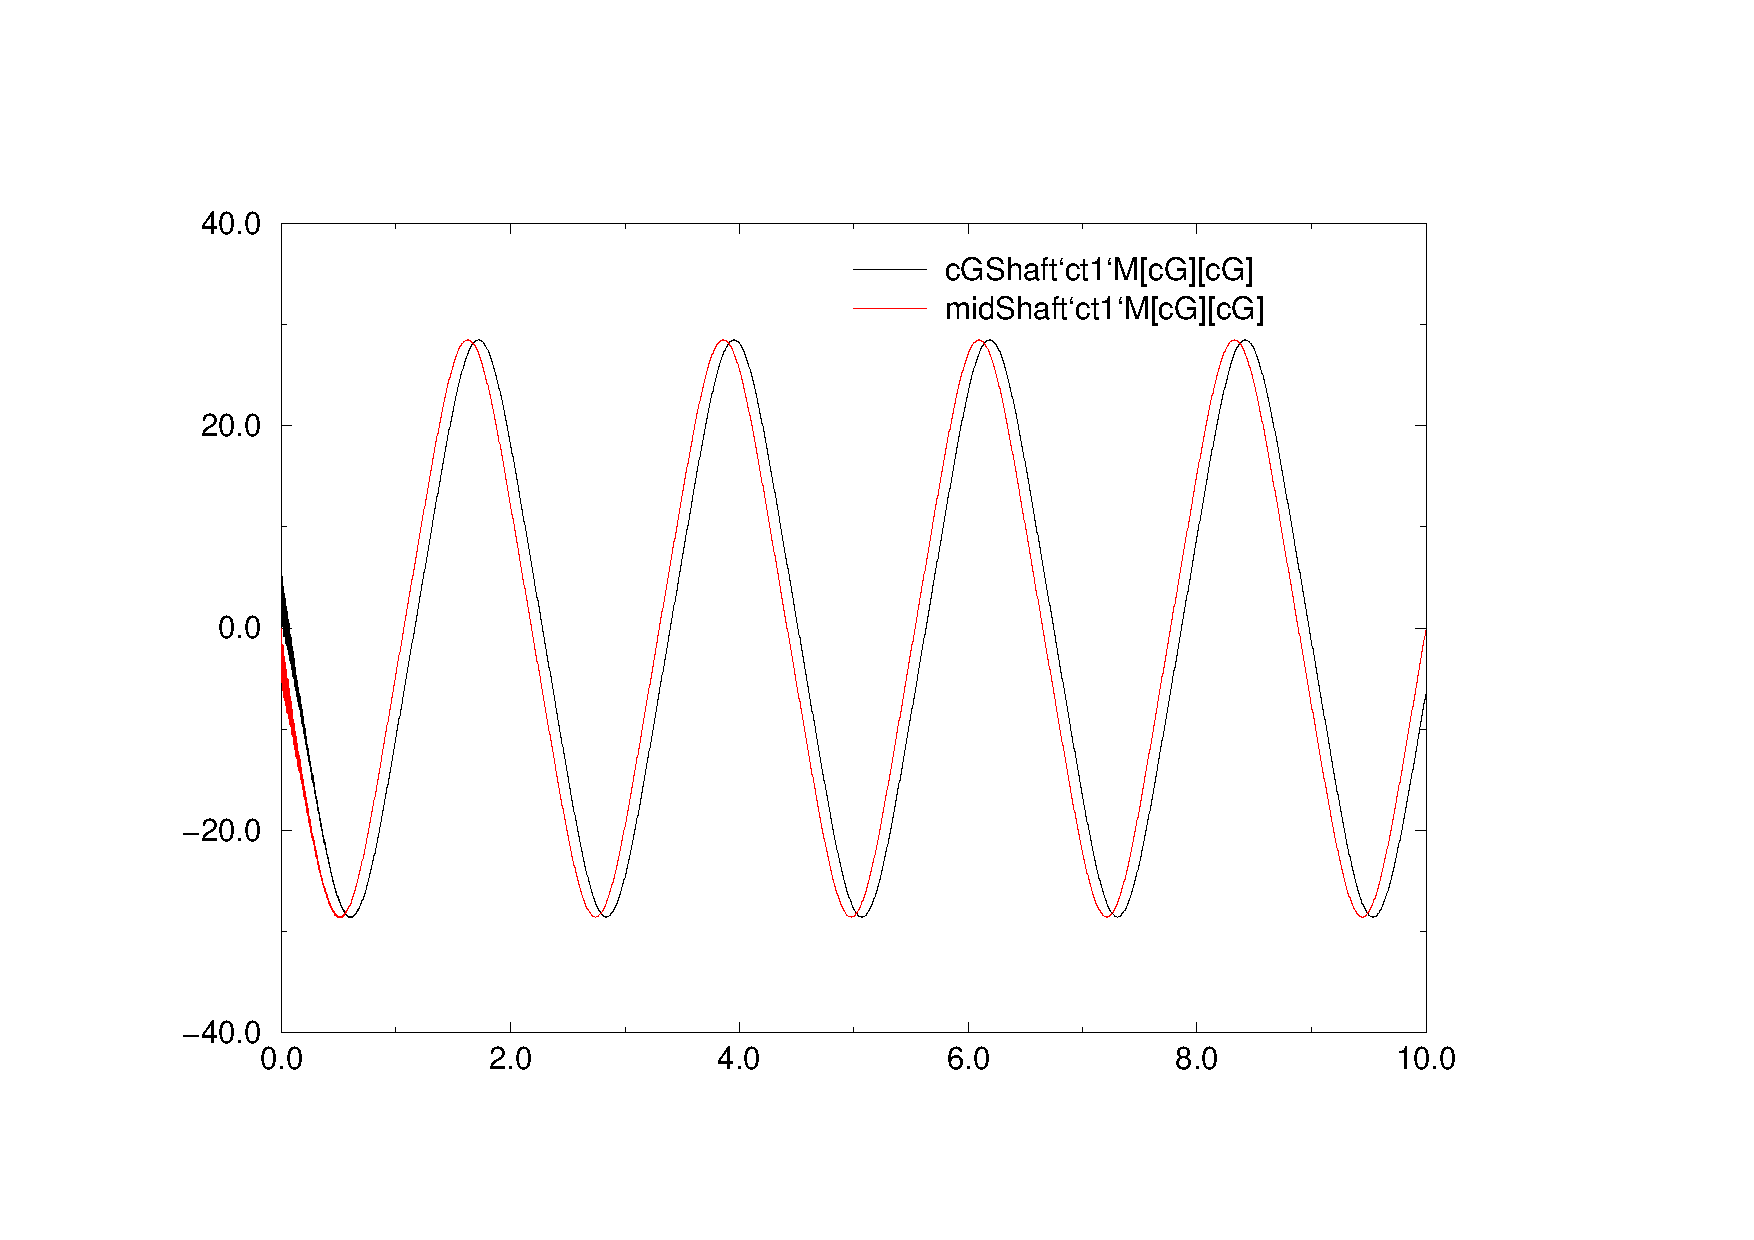
\includegraphics[width=6cm]{figs/S1S2_M.pdf}}
	\label{fig:MomenatcGShaftmidShaft}
	}
\subfigure[Moment in TLM connected coordinate systems midShaft-endShaft.]{
	{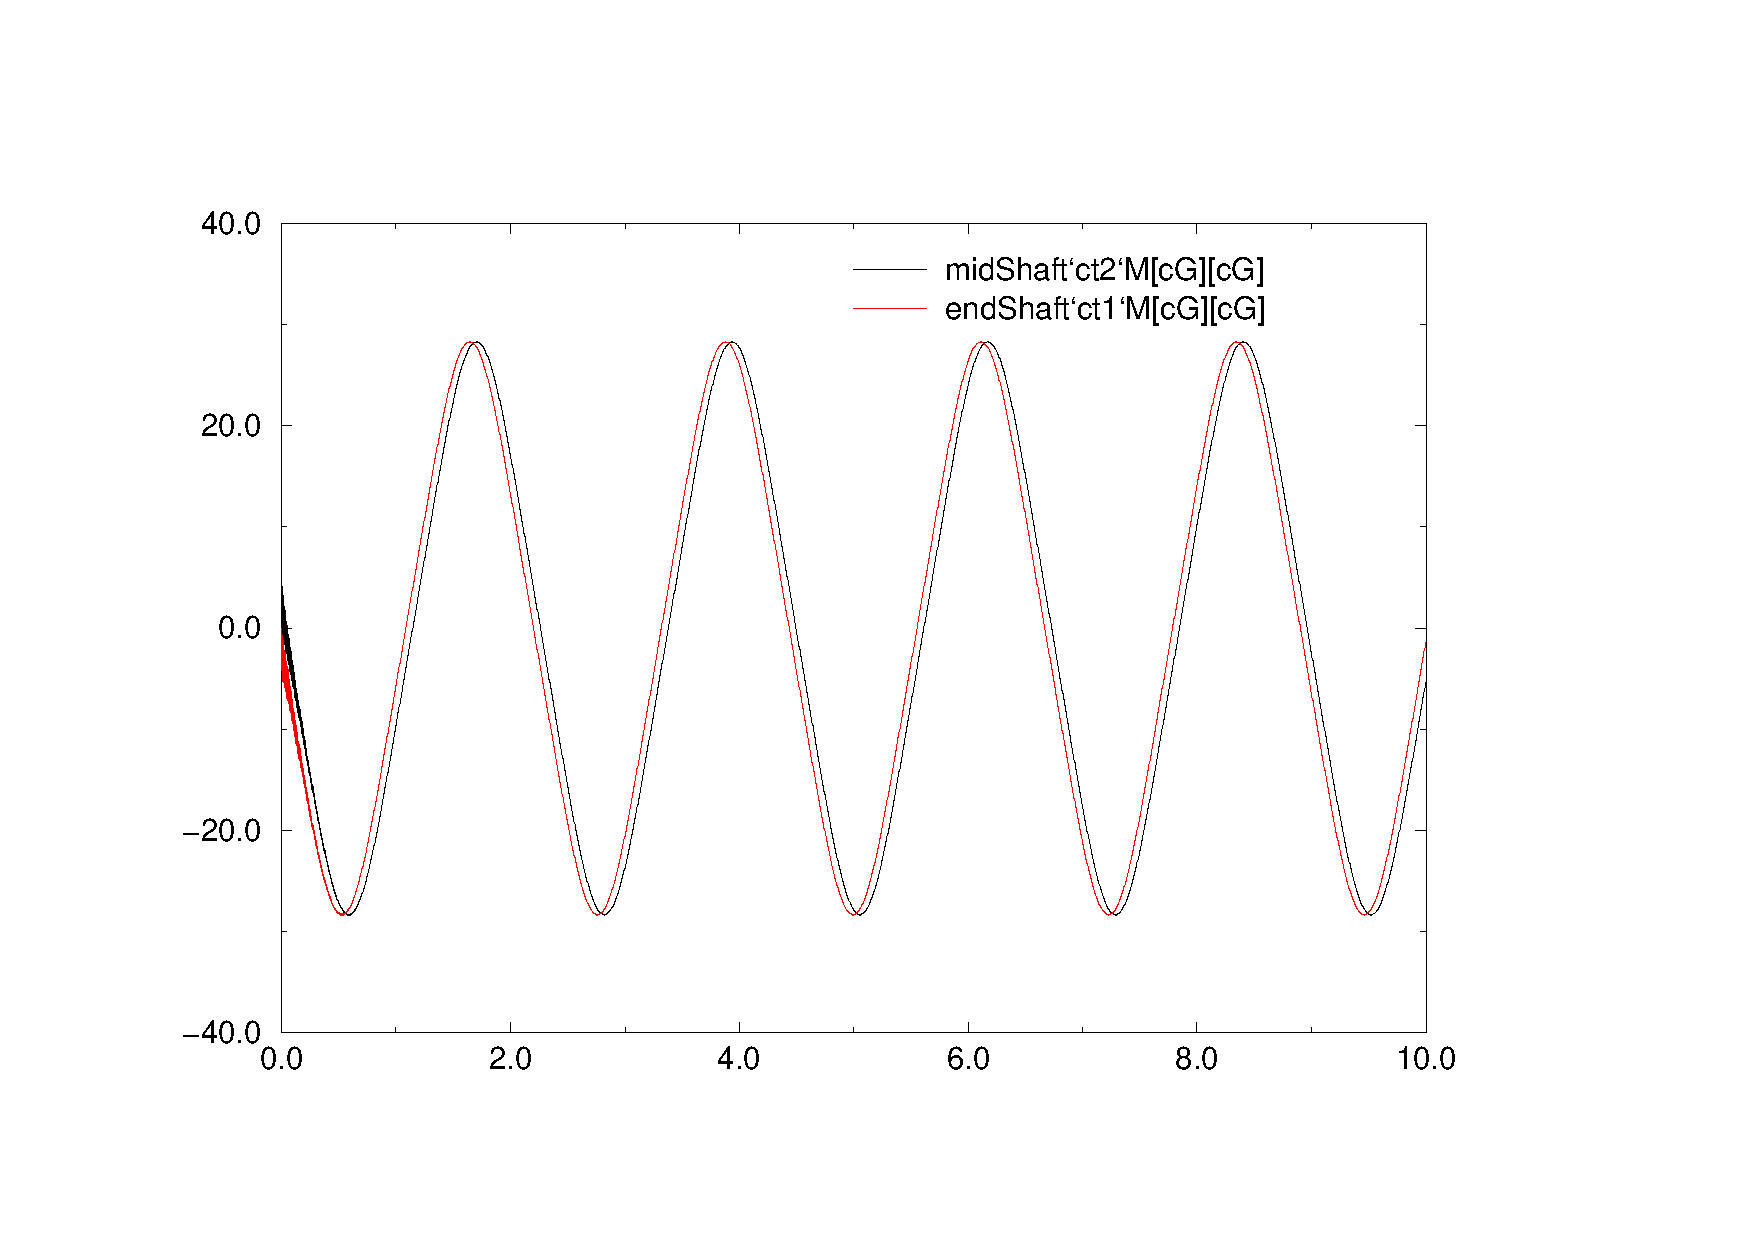
\includegraphics[width=6cm]{figs/S2S3_M.pdf}}
	\label{fig:MomentmidShaftendShaft}
     	}	
\caption{The difference in Moment between the TLM connected coordinate
	systems due to TLM delay.}
\label{fig:MomentShafts}
\end{figure}

Figure~\ref{fig:MomentShafts}, for instance, shows the moments created in the TLM interfaces of the connected Simulink models. 
One can nicely see the time delay in the connected interfaces due to TLM delay.

\section{Installation}
Generally the following steps need to be conducted for a correct installation of the plugin:
\begin{enumerate}
\item Install the plugin files on your system.
\item Add the installation directory or directories to the Matlab {\tt Search Path}.
\item Possibly adjust the StartTLMSimulink start-up script to your needs.
\end{enumerate}

The Simulink TLM-plugin consists of three files:
\begin{itemize}
\item A tlmforce S-Function, or tlmforce.mex* file.
\item A TLM library file, TLMLib.mdl.
\item A start-up script, StartTLMSimulink
\end{itemize}

The start script is located in the {\tt bin} directory in the TLMSimulator folder. 
The tlmforce S-Function mex and the TLMLib.mdl files are placed in the {\tt bin/\$ABI/Simulink} directory. 
There is a Linux and a MS-Windows version of the plugin available.

It is important that the TLMLib.mdl and tlmforce.mex* file are within the Matlab {\tt Search Path}. 
This can be achieved with the {\tt Select Path} dialog that can be opened from the {\tt File} menu in the Matlab main window.

Changes to the StartTLMSimulink script are typically not necessary. 
Note that there are two versions of the script, a MS Windows batch script and a c-shells script for Linux/Unix
systems. 
In case the system requires a special setup for running Matlab/Simulink it is recommended to make changes to the script. 
Below is the c-shell version of the script:
\begin{verbatim}
#!/bin/csh -f

setenv PATH ${PATH}:/home/alex/bin/matlab2006b/bin
set SIMCOMMAND="matlab -nosplash -nodesktop -nojvm -r"

#############################################################
#------ Changes below this line should not be needed     ----

if("a$1" == "a") then
echo This script is used by TLM manager to start simulations
echo It should result in a call to matlab/simulink
exit 1
endif

cd $1

echo Starting a simulation with input file: $6
echo Make sure that:
echo time = $2
echo timeEnd = $3
echo MaxTimeStep "<"= $4
echo Writing component name $1 and server name $5 to file tlm.config
echo $1 $5 > tlm.config
echo $2 $3 $4 >> tlm.config

echo Starting matlab/simulink
echo $SIMCOMMAND

echo Writing execution methods to runtlm.m
echo "$6;" > runtlm.m
if( "$4" != "0" ) then
 echo "opts = simset('MaxStep', $4);" >> runtlm.m
 echo "sim( '$6', [$2 $3], opts );" >> runtlm.m
else
 echo "sim( '$6', [$2 $3] );" >> runtlm.m
endif
echo "save; quit force;" >> runtlm.m

exec $SIMCOMMAND runtlm > ${6}.simlog
\end{verbatim}


\section{Creating External Simulink Models}
To enable an existing Simulink model for co-simulation is fairly simple:
\begin{enumerate}
\item Open the model and the TLM library TLMLib.mdl, see also Figure~\ref{fig:TLMLib}.
\item Drag the TLMForce (pure Simulink) or TLMInterface (SimMechanics) block into the model.
\item Create the necessary connections to the TLM block, see also Section~\ref{sec:TLMLib} for details about signal dimensions.
\item Send all signals of interest to the Matlab workspace or to a file.
\end{enumerate}

Remember, that the TLM plugin requires velocities to calculate output force and moment. 
Remember also, that all data must be expressed relative the global inertial system. 
Necessary coordinate transformations should be implemented in the Simulink model.

All external models are automatically executed on co-simulation start-up and terminated when the simulation is finished. 
Data that is not written to a file is lost when the simulation terminates. 
The Simulink plugin writes Matlab workspace content to the file {\tt matlab.mat} when the simulation is
finished. 
All simulation data that should be analyzed should either be written to a file during the simulation or stored in the workspace. 
The latter can be achieved by using a Simulink {\tt ToWorkspace} sink, by logging signals, or by logging Simulink {\tt Scope} data.

The next step is to create an external model from the TLM prepared Simulink model. 
It is created using the composite model editor. 
The composite model describes how different external models are connected and what TLM parameters should be used in the different TLM
connections. 
Creating external Simulink models is not different from creating any other external model. 
Only the correct start-up method, i.e., StartTLMSimulink needs to be selected.

{\em NOTE:} Neither Simulink nor SimMechanics can export surface graphics for visualization of the composite model. 
Graphics files, i.e., VRML or STL files, can be created from a CAD tool or with the Virtual-Reality authoring tool of the Matlab Virtual Reality toolbox.

Results from the co-simulation can be verified in CME by plotting the movement of the TLM interfaces.
